\chapter{Formatting}

\section{Figures and Tables}
Figures and tables need to include a caption. This can be done with the LaTeX-command \texttt{\bslash caption$\lbrace\rbrace$}. To be able to reference figures and tables, a \texttt{\bslash label$\lbrace\rbrace$} must follow the caption.

\begin{figure}[h!]
  \begin{center}
    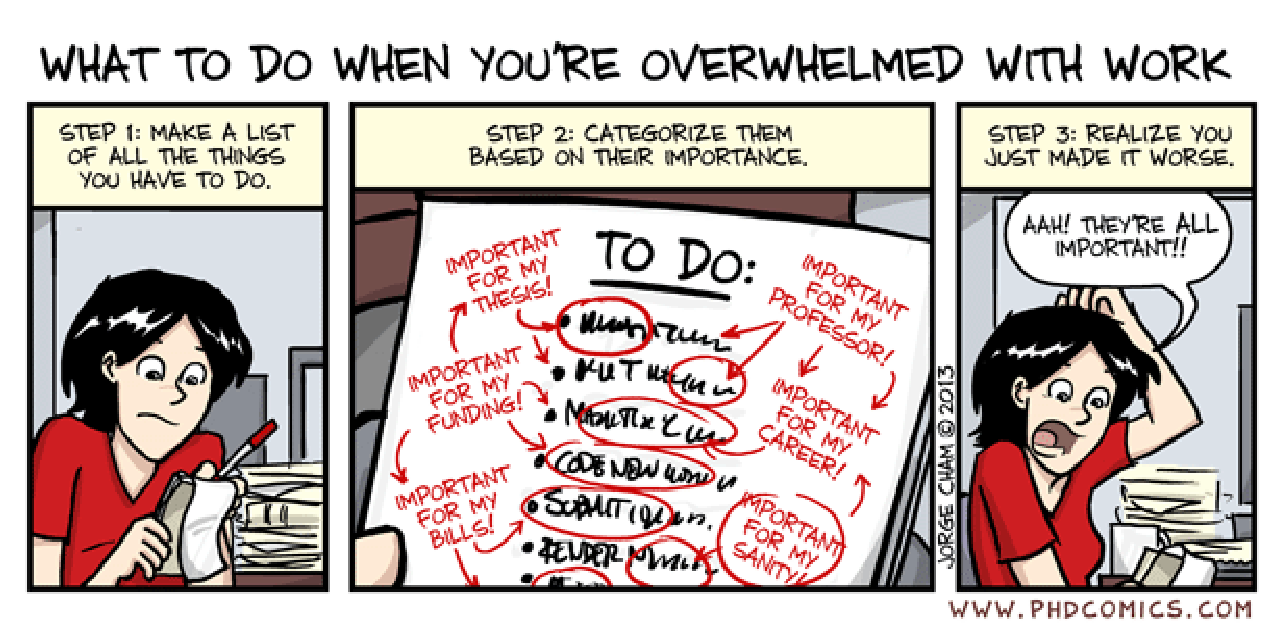
\includegraphics[width=0.6\textwidth]{phd112013s.eps}
    \caption{Ein PHD Comic}
    \label{fig:ToUseWithReference}
  \end{center}
\end{figure}

\begin{table}[b]
\begin{center}
\begin{tabular}{|l |c|}
\hline 
\textbf{Parameter} & \textbf{Value} \\
\hline  
\hline 
Transmission Power & 23~dBm\\
\hline 
Center Frequency & 2.6~GHz\\
\hline 
Channel Bandwidth & 15~kHz\\
\hline 
Shadowing Correlation Distance & 40~m\\
\hline 
Noise Density & -174~dBm/Hz\\
\hline 
Antenna Heights & 1.5~m\\
\hline 
\end{tabular}
\caption{Simulation Parameters and Values}\label{tab:param_table}
\end{center}
\end{table}

The labelled figures and tables can be referenced via \texttt{\bslash ref}, e.g. ~Figure~\ref{fig:ToUseWithReference}.
\newpage

\section{Referencing}
Literature references are included e.g. like this:\\
``..., as shown in \cite{eberspaecher97},, ...'' or ``... there are several approaches \cite{arnaud99,griswold90} ...''